\subsection{A LIfe Question}
\begin{frame}[t]{A Life Question [JH p25] [RH p18] }
\begin{columns}[T, onlytextwidth]
\column{0.5\textwidth}
The \Sun\ (L1) and \Moon\ are both VOC, with the \Moon\ being first to leave her sign so looked to her first with the \Sun\ as sharer.\\
\vspace{0.25cm}
\Moon\ 28 \Aries\ $\Rightarrow$ \Taurus \\
\hspace{1em}$\Rightarrow$ \Square\ \Mercury\ 2 \Taurus\ - \Moon\ commits her disposition \\
\hspace{1em}\Mercury\ $\Rightarrow$ \Sextile\ \Saturn\ 4 \Aquarius\ with reception \\
therefore \Saturn\ signifies the person's health and good fortune because he's in his own domicile \\
\vspace{0.25cm}
\Sun\ 24 \Aquarius\ $\Rightarrow$ \Pisces \\
\hspace{1em}$\Rightarrow$ \Sextile\ \Jupiter\ 9 \Pisces \\
even though \Jupiter\ is L8, the \Sextile\ is in \Jupiter's domicile, so he receives the \Sun, and the \Sun\ (as L1) signifies health and good fortune \\
\vspace{0.25cm}
Both L1 and the \Moon\ indicate the same for the person's health and fortune.
\column{0.5\textwidth}
\begin{center}
{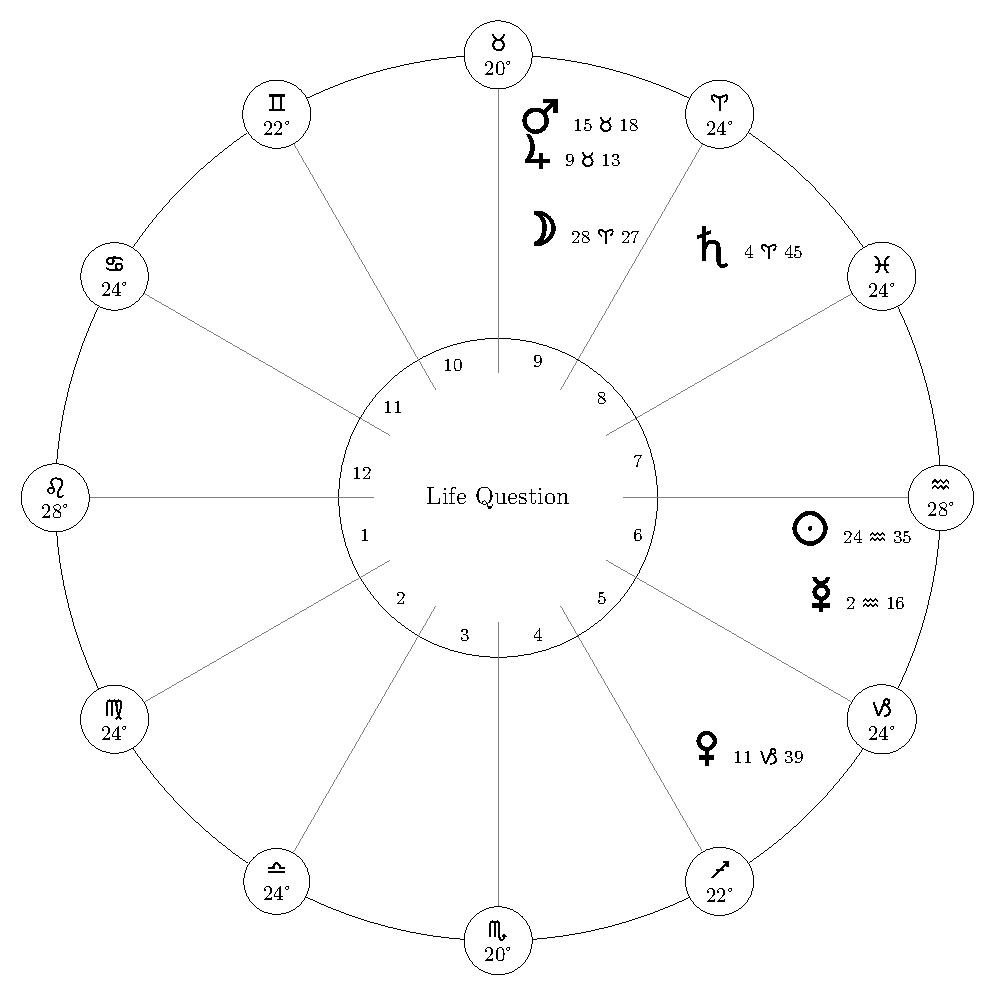
\includegraphics[width=0.9\textwidth]{charts/22-chart-life}}
\end{center}
\end{columns}
\end{frame}
% -------------------------------------------------------
\begin{frame}[t]{A Life Question Continued}
\begin{columns}[T, onlytextwidth]
\column{0.5\textwidth}
Wanting to know when the sickness would lessen, Masha'allah says he next looked at the House of Sickness, the 6th, which was ruled by \Saturn, who, being the heaviest, was not separating or joining any planet; so he looked for who was applying or separating from \Saturn, and found: \\

\vspace{0.25cm}
\Venus\ (11 \Capricorn) was separated from \Saturn\ by 7° and \\
\hspace{1em}$\Rightarrow$ \Trine\ \Mars\ (15 \Taurus) \\ 
with each receiving the other; \Mars\ receiving \Venus\ in his exaltation, \Venus\ receiving \Mars\ in her domicile.\footnote{Here, the sign occupied by \Mars\ is used to define the reception rather than the sign the aspect falls in, which was the case in the previous example.}\\

\vspace{0.25cm}
This \textsl{"signified a lessening of pain and the arrival of health"}
\column{0.5\textwidth}
\begin{center}
{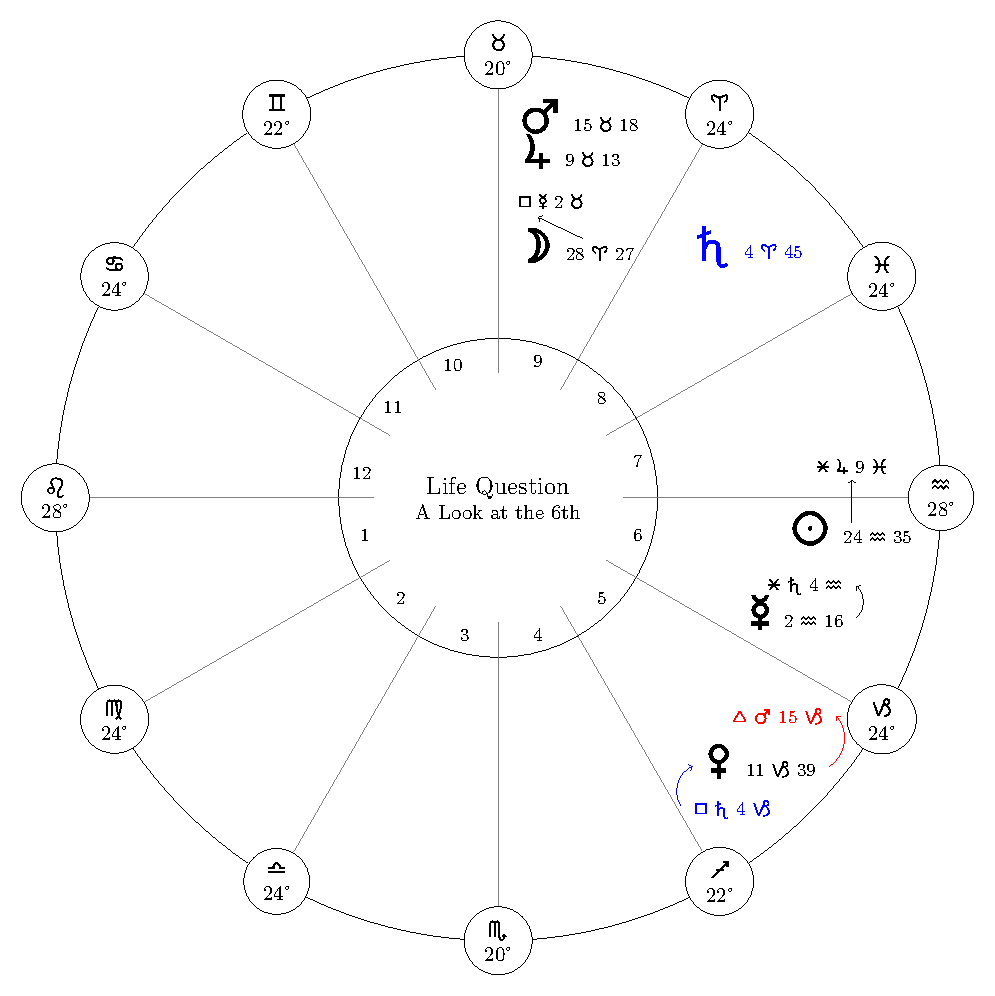
\includegraphics[width=0.9\textwidth]{charts/22a-chart-life}}
\end{center}
\end{columns}
\end{frame}